%
%
%            -----  The Scout Programming Language -----
% 
%  This file is distributed under an open source license by Los Alamos
%  National Security, LCC.  See the file License.txt (located in the
%  top level of the source distribution) for details.
%  
% -----
% 
%  $Revision$
%  $Date$
%  $Author$
%
% -----
% 
% Useful build command: latexmk --pdf reference
% 
\documentclass[10pt,letterpaper,extrafontsizes]{memoir}
\usepackage{fourier,etex,fixltx2e,alltt,xcolor,latexsym}
\usepackage{dpfloat,url,color,calc,graphicx,soul,fourier} 
\usepackage{fonttable}
\usepackage{layouts}

\usepackage{color,calc,graphicx,soul,fourier,scout}
\usepackage[pdftex, bookmarks, colorlinks=true, linkcolor=blue,
   pdftitle={Combustion Exascale Co-Design Center -- Work Breakdown Structure}
   pdfsubject={CECDC -- Work Break-down Structure}]{hyperref}



\makeatletter
\newlength\dlf@normtxtw
\setlength\dlf@normtxtw{\textwidth}
\def\myhelvetfont{\def\sfdefault{mdput}}
\newsavebox{\feline@chapter}


\setlength{\parskip}{1\baselineskip}
\setlength{\parindent}{0pt}

\newcommand\feline@chapter@marker[1][4cm]{%
  \sbox\feline@chapter{%
    \resizebox{!}{#1}{\fboxsep=0.85pt%
      \colorbox{scoutblue}{\color{white}\bfseries\sffamily\thechapter}%
    }}%
  \raisebox{\depthof{\usebox{\feline@chapter}}}{\usebox{\feline@chapter}}%
}

\newcommand\feline@chm[1][4cm]{%
  \sbox\feline@chapter{\feline@chapter@marker[#1]}%
  \makebox[0pt][l]{% aka \rlap
    \makebox[1cm][r]{\usebox\feline@chapter}%
  }}
\makechapterstyle{daleif1}{
  \renewcommand\chapnamefont{\normalfont\Large\scshape\raggedleft\so}
  \renewcommand\chaptitlefont{\normalfont\huge\bfseries\scshape\color{scoutblue}}
  \renewcommand\chapternamenum{}
  \renewcommand\printchaptername{}
  \renewcommand\printchapternum{\null\feline@chm[2.25cm]}
  \renewcommand\afterchapternum{\hskip 1.5cm} %\par\vskip\midchapskip}
  \renewcommand\printchaptertitle[1]{\chaptitlefont ##1\par}
  \renewcommand{\afterchaptertitle}{\par\nobreak\medskip\hrule\vskip\afterchapskip}
}
\makeatother
\chapterstyle{daleif1}

\newcommand*{\titleSC}{\begingroup% Misericords, T&H p 153
%\tdrop=0.08\txtheight\centering\vspace*{\tdrop}
\centering
{\LARGE \scshape The Scout Programming Language}\\[\baselineskip]
{\Huge\bfseries Language Reference}\\[\baselineskip]

\includegraphics{images/scout-logo.pdf}
{\flushleft 
\includegraphics[width=1.0in]{images/lanl-logo.pdf} \hfill 
 Version 1.0 -- March 2015}\par
\vfill
\endgroup}

\begin{document}
\pagenumbering{roman}
\pagestyle{headings}
\pagestyle{empty}
\titleSC
\clearpage

% copyright page                                                                                              
\begingroup
\footnotesize
\setlength{\parindent}{0pt}
\setlength{\parskip}{\baselineskip}
%%\ttfamily

Copyright \textcopyright{} 2010. Los Alamos National Security,
LLC. This software was produced under U.S. Government contract
DE-AC52-06NA25396 for Los Alamos National Laboratory (LANL), which is
operated by Los Alamos National Security, LLC for the U.S. Department
of Energy. The U.S. Government has rights to use, reproduce, and
distribute this software.  NEITHER THE GOVERNMENT NOR LOS ALAMOS
NATIONAL SECURITY, LLC MAKES ANY WARRANTY, EXPRESS OR IMPLIED, OR
ASSUMES ANY LIABILITY FOR THE USE OF THIS SOFTWARE.  If software is
modified to produce derivative works, such modified software should be
clearly marked, so as not to confuse it with the version available
from LANL.

Additionally, redistribution and use in source and binary forms, with
or without modification, are permitted provided that the following
conditions are met:

\begin{itemize}

  \item Redistributions of source code must retain the above copyright
    notice, this list of conditions and the following disclaimer.

  \item Redistributions in binary form must reproduce the above
    copyright notice, this list of conditions and the following
    disclaimer in the documentation and/or other materials provided
    with the distribution.

  \item Neither the name of Los Alamos National Security, LLC, Los
    Alamos National Laboratory, LANL, the U.S. Government, nor the
    names of its contributors may be used to endorse or promote
    products derived from this software without specific prior written
    permission.
\end{itemize}


THIS SOFTWARE IS PROVIDED BY LOS ALAMOS NATIONAL SECURITY, LLC AND
CONTRIBUTORS ``AS IS'' AND ANY EXPRESS OR IMPLIED WARRANTIES,
INCLUDING, BUT NOT LIMITED TO, THE IMPLIED WARRANTIES OF
MERCHANTABILITY AND FITNESS FOR A PARTICULAR PURPOSE ARE
DISCLAIMED. IN NO EVENT SHALL LOS ALAMOS NATIONAL SECURITY, LLC OR
CONTRIBUTORS BE LIABLE FOR ANY DIRECT, INDIRECT, INCIDENTAL, SPECIAL,
EXEMPLARY, OR CONSEQUENTIAL DAMAGES (INCLUDING, BUT NOT LIMITED TO,
PROCUREMENT OF SUBSTITUTE GOODS OR SERVICES; LOSS OF USE, DATA, OR
PROFITS; OR BUSINESS INTERRUPTION) HOWEVER CAUSED AND ON ANY THEORY OF
LIABILITY, WHETHER IN CONTRACT, STRICT LIABILITY, OR TORT (INCLUDING
NEGLIGENCE OR OTHERWISE) ARISING IN ANY WAY OUT OF THE USE OF THIS
SOFTWARE, EVEN IF ADVISED OF THE POSSIBILITY OF SUCH DAMAGE.
\endgroup

\clearpage
 

\tableofcontents
\setlength{\unitlength}{1pt}
\clearpage
\listoffigures
\clearpage
\listoftables
\lstlistoflistings

%\clearpage
%\listofegresults

\chapter*{Preface}

\textsf{scout \textsl{verb} [intrans.] -- \textit{to explore or examine so as to gather
information.}}
\vskip 0.25in

\section*{Welcome}
The goal of this manual is to provide you with a quick reference to the syntax, 
semantics and features of the experimental Scout language.  We assume that the
reader is an experienced programmer with a basic understanding of parallel 
computing.  Although we do our best to keep the language documentation up to 
date with the feature set supported by the open-source versions of Scout, readers
are encouraged to look over the release notes provided with each version for 
important details.

\section*{About Source Code Listings}

The source code listings in this manual uses both font changes and \textit{syntax aware} 
coloring that helps the reader to identify parts of the language.  Table~\ref{src_listing_table}
provides a key to the font and colors using in the listings. 

\begin{table}
  \begin{center}
  \begin{tabular}{| l | l | l |}
    \hline
 	\textsc{Type}      & \textsc{Color}                           & \textsc{Font}     \\ \hline 
	\textsc{keywords}  & {\texttt{\color{keywordcolor}keyword}}   & \texttt{keyword}  \\ \hline 
    \textsc{built-ins} & {\texttt{\color{builtincolor}built-ins}} & \texttt{built-in} \\ \hline 
    \textsc{comments}  & {\textit{\color{commentcolor}comments}}  & \textit{comments} \\ \hline 
    \textsc{strings}   & {\textit{\color{stringcolor}"string"}}   & \textit{"string"} \\ \hline 
  \end{tabular}
  \end{center}
  \caption{Source code listing colors and fonts.}
  \label{src_listing_table} 
\end{table}


\section*{Support}
If you have questions, or encounter problems, please feel free to send an email
to the Scout support team via email: {\color{scoutblue}scout-support@lanl.gov}.

\section*{Open Source Effort}
This version of Scout is an open-source software effort established by Los Alamos
National Laboratory's Applied Computer Science Group.  If you are interested in 
joining the development team please visit our web site for more details:
\begin{center} 
	{\color{scoutblue}\url{http://www.need-a-scout-url-here.com}}.
\end{center}







\clearpage
\pagenumbering{arabic}
\let\clearforchapter\par % cheating, but saves some space

\chapter{Introduction}

Scout is an experimental programming language that combines
sequential, task- and data-parallel computing constructs along with a
set of specialized constructs for the visualization and analysis of
data. In addition, the language exposes a set of \emph{first-class}
data types that represent a variety of computational meshes.  These
features are provided via extensions to the C programming language.
In this manual we assume the reader is familiar with some of the basic
ideas behind parallel programming and fully familiar with the C
language.  This chaper provides a high-level introduction to the
compiler, data types, and language constructs -- more complete details
of each of these topics is provided in the remaining chapters.

\section{Scout and the C Programming Language}
\label{ch1:scout-clang}

Scout extends the C programming language to support a new set of
abstractions and domain-specific constructs.  Some of the main
domain-specific constructs in Scout are explicit mesh declarations,
instantiations and parallel computation over the various components of
the mesh (e.g. cells, vertices, edges) or over array elements.  Scout
builds upon the fundamental types of C to include higher-level
abstractions -- such as computational meshes and the associated fields
stored on a mesh.  From this perspective, Scout is a higher-level
language than C.

Since Scout is based on the open-source Clang and LLVM Compiler Infrastructure, all of 
the C language features are available. 
Scout extends the fundamental data types
available in C to include vector types of two, three, and four components.  Scout's 
syntax for vector types follows closely with those used by the OpenGL Shading Language
and NVIDIA's C for CUDA.  Section~\ref{ch:datatypes} below covers these topics in more 
detail.

\section{Getting Started}
\label{ch1:started}

The best way to learn any programming language is to get your hands dirty.  The classic
{hello world} program does not need to rewritten for Scout, since Scout fully supports
C.  Therefore, as an introductory program to Scout, Listing~\ref{lst-forallmesh}  
illustrates a simple one-dimensional mesh transformation.  It uses the \texttt{mesh}
abstraction, the mesh's associated fields and the parallel \texttt{forall} construct.

\par\bigskip
\begin{lstlisting}[label=lst-forallmesh,caption={Simple mesh example.}]
uniform mesh MyMesh{
  cells:
    float a;
    float b;
    float sum;
};

int main(int argc, char** argv){

  MyMesh m[512];

  // initialization of a and b not shown

  forall cells c in m {
    sum = a + b;
  }

  return 0;
}
\end{lstlisting}
\par\bigskip\noindent

\section{Compiling a Scout Program}
\label{ch1:compiling}

Scout's compiler follows the characteristics of traditional (Unix) command line interfaces.  In 
the following example, the simple mesh program from Listing~\ref{lst-forallmesh} is compiled and 
executed from the command prompt:

\par\bigskip
\fcolorbox{scoutblue}{lightgray}{
  \parbox{\textwidth-10pt}{%
    \texttt{\small \$ scc simplemesh.sc} \cmdcmt{compiler produces default executable ''a.out''...}\\      
    \texttt{\small \$ ./a.out}\\
    \texttt{\small \$ \_ }
  }
}
\par\bigskip\noindent

The previous compilation of the Scout program creates an executable that is targeted to run
sequentially on a CPU.  

%Scout can also be enabled to run CPU multithreading via the \texttt{-mt}
%option to \texttt{scc} or run on an NVIDIA GPU via the \texttt{-gpu} option to \texttt{scc}.

Scout can be enabled to run on an NVIDIA GPU via the \texttt{-gpu} option to \texttt{scc}.

% Do we have an scc man page anywhere?
%See the on-line \texttt{scc} man page, or Appendix~\ref{app-scc} for more information on the
%available command line options.

See the output to \texttt{scc -help} or Appendix~\ref{app-scc} for more information on the
available command line options.
 % introduction 
\clearpage
\let\clearforchapter\par % cheating, but saves some space


\chapter{Data Types}
\label{ch:datatypes}


Those familiar with programming in C should find Scout's syntax and fundamental data 
types to be very familiar.  In this section we quickly review Scout's additional composite data types.

\section{Vectors}
\label{ch:vectors}

As briefly mentioned in Section~\ref{ch1:scout-clang}, Scout provides support for two-, three-, 
and four-component vector types.  The "base" type for vectors includes signed and unsigned 
values of each of the fundamental types (\texttt{bool}, \texttt{char}, \texttt{short}, 
\texttt{int}, \texttt{long}, \texttt{float}, \texttt{double}).  The syntax for defining a 
vector uses these types followed by the number of components in the vector. Listing~\ref{lst-vector} 
shows some example vector declarations and initializations.

\par\bigskip
\begin{lstlisting}[float=h,label=lst-vector,
    caption={Vector declarations and initialization.}]
// Vector declarations
float2  u; // two-component single-precision vector.
int3    v; // three-component integer vector.
double4 w; // four-component double-precision vector.

// Vector declaration and initialization
float3 foo = (float3){1.0f, 2.0f, 3.0f};

// Another way to initialize a vector
float4 bar;
bar.x = 1.0f;
bar.y = 2.0f;
bar.z = 3.0f;
bar.w = 4.0f;
\end{lstlisting}
\par\bigskip\noindent

\section{Meshes}
\label{ch:meshes}

Computational science data structures are frequently based on the concept of a mesh.
Scout directly follows this philosophy by introducing mesh-centric data types.  Scout supports 
the \texttt{uniform} mesh type.  

%\texttt{rectilinear}, \texttt{structured}, and \texttt{unstructured} 

In addition, the language 
provides constructs for defining the values stored on the various locations of the mesh (e.g.
cell centers, vertices, edges and faces).  Figure~\ref{fig:types:mesh-def} illustrates the layout of a mesh.
Figure~\ref{fig:types:grid-positions} shows the field placement options within a mesh.

\par\bigskip
\begin{figure}[h]
  \centering
  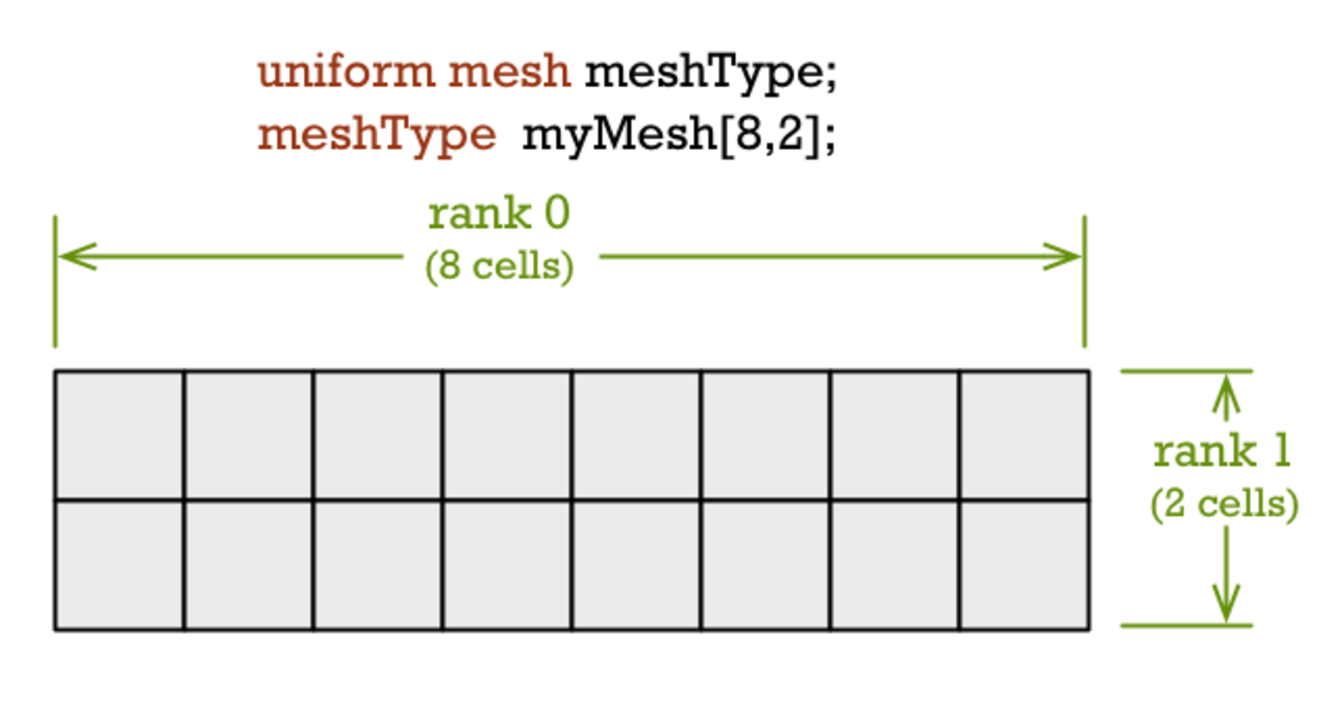
\includegraphics[width=4.0in]{datatypes/figures/mesh-def.pdf} \\
  \caption{Example of a uniform mesh definition.}
  \label{fig:types:mesh-def}
\end{figure}



\begin{figure}[h]
  \centering
  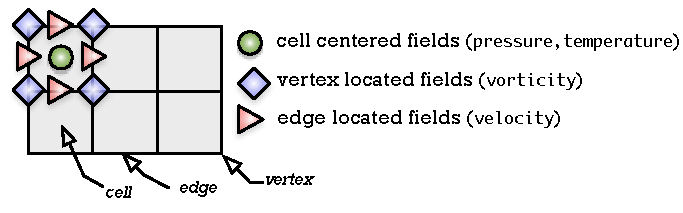
\includegraphics[width=4.0in]{datatypes/figures/field-positions.pdf} \\
  \caption{Field placement options within a mesh.}
  \label{fig:types:grid-positions}
\end{figure}
\par\bigskip\noindent

%TODO:  need a 2D picture that shows faces.

Here is a code example showing a two-dimensional mesh and a mesh
whose dimensions are defined by an input file.
Listing~\ref{lst-mesh} shows some example mesh declarations.
Note that is is not yet implemented to read meshes from input files.

\par\bigskip
\begin{lstlisting}[float=h,label=lst-mesh,
    caption={Mesh declarations.}]
// Two-dimensional uniform mesh with values stored at cell 
// centers and cell verticies. 
uniform mesh MeshType {
	cells:    float temperature;
	          float presure;
	vertices: float3 vorticity;
  edges:    float  velocity;
};

MeshType myMesh[512,512];

\end{lstlisting}
\par\bigskip\noindent


In addition, meshes dimensions can be specified using variables.
Listing~\ref{lst-meshvar} shows this.

\par\bigskip
\begin{lstlisting}[float=h,label=lst-meshvar,
    caption={Mesh declarations using variable.}]
  int dim = 4;

  uniform mesh HeatMeshType{
  cells:
    float t1, t2;
  };

  HeatMeshType heat_mesh[dim];
\end{lstlisting}
\par\bigskip\noindent


%Note: need examples here of how to declare rectilinear, structured and unstructured meshes.
 % data types
\clearpage
\let\clearforchapter\par % cheating, but saves some space


\chapter{Parallel Constructs}

\section{Data-parallel Operations}

\subsection{\texttt{forall} Loops for Meshes}

Building upon the mesh data types, Scout provides support for parallel computations over the 
elements/attributes of the mesh (cells, vertices, etc.).  The majority of these constructs 
use an explicit parallel form that is mixed with the main body of the code that is, by 
definition, executed sequentially.  

Listing~\ref{lst-forall} shows an example parallel 
\texttt{forall} construct.  In this case we are looping over all the cells of the mesh 
\texttt{myMesh} and setting the values of the cell attributes (\texttt{a} and \texttt{b})
to $0.0$.  Note that we can use the specified cell placeholder "\texttt{c}" to directly
access the attributes of the currently active cell using a C-like structure member access
notation.  If there are no clashes within scope, the use of the of explicit cell deferencing
may be dropped within the body of the loop (e.g. \texttt{c.a = 0.0;} can be replaced with
\texttt{a = 0.0f;}).

\par\bigskip
\begin{lstlisting}[float=t,label=lst-forall,
	caption={A \texttt{forall} loop construct.}]
	uniform mesh MeshType {
		cells: float a, b;
	};
  MeshType myMesh[16];

	forall cells c in myMesh { // 'c' is the active cell.
		c.a = c.b = 0.0f;
}
\end{lstlisting}
\par\bigskip\noindent

Note that the code in the body of a \texttt{forall} construct must follow some
constraints.  A field inside a \texttt{forall} construct body may only be
read-only or write-only code that does not satisfy this condition is rejected by the compiler. 
This limitation significantly reduces the complexity of analyzing data dependencies between 
parallel constructs.  Another constraint is that if targeting the GPU, instructions for printing
within the \texttt{forall} construct are not allowed.  Lastly, variables declared outside
of the \texttt{forall} construct body cannot be assigned to within the \texttt{forall}
construct body.

Additional levels of parallelism can be introduced by nesting parallel constructs.  
Specifically, the parallel operations over the cells of a mesh can be combined with  
with a set of operations over the components of each individual cell. Listing~\ref{lst-nestforall} 
shows such a nesting.  

\par\bigskip
\begin{lstlisting}[float=h,label=lst-nestforall,
	caption={Nested \texttt{forall} loop construct over mesh components.}]
forall cells c in myMesh { // 'c' is the active cell.
	forall vertices v in c { // 'v' is the active vertex.
	  c.a += v.a * v.a;
	}
	c.a = sqrt(c.a);
}
\end{lstlisting}
\par\bigskip\noindent

Note that up to two levels of \texttt{forall} nesting are supported.  The complete listing of all two-level nested combinations is shown in Listing~\ref{lst-all-nestforall} .

\par\bigskip
\begin{lstlisting}[float=h,label=lst-all-nestforall,
	caption={All supported two-level nested \texttt{forall} loop constructs over mesh components.}]
forall edges e in m {
  forall cells c in e {}}

forall edges e in m {
  forall vertices v in e {}}

forall faces f in m {
  forall cells c in f {}}

forall vertices v in m{
  forall cells c in v {}}

forall cells c in m {
  forall edges e in c {}}

forall cells c in m {
  forall faces f in c {}}

forall cells c in m {
 forall vertices v in c {}}
\end{lstlisting}
\par\bigskip\noindent

% TODO Dean -- did I forget any?  Also, does this work for query?

The \texttt{position()} built-in function of a cell is automatically provided to contain the coordinates of the
current cell being processed. Listing~\ref{lst-position-forall} shows how positions can be
used.

\par\bigskip
\begin{lstlisting}[float=h,label=lst-position-forall,
	caption={Accessing the position of cells within \texttt{forall} loop construct.}]
forall cells c in heat_mesh {
  if (c.position().x > 0 && c.position().x < 1023)
    t1 = 0.0f;
  else
    t1 = MAX_TEMP;      
}
\end{lstlisting}
\par\bigskip\noindent

The \texttt{width()}, \texttt{height()}, \texttt{depth()} and \texttt{rank()} 
built-in functions are provided to enable
the user to obtain the width, height, depth or rank of the mesh within a \texttt{forall} or outside of one.  
When using the built-in functions outside of a \texttt{forall}, the mesh variable is given as an argument
to the built-in function.  When used within a forall, the cell can be given as an argument or no argument 
need be specified.
Listing~\ref{lst-dims} shows how the dimension built-in functions can be used.

\par\bigskip
\begin{lstlisting}[float=h,label=lst-dims,
	caption={Accessing the dimensions of a mesh.}]
uniform mesh MyMesh {
 cells: 
  float a;
};

MyMesh m[3,4];
assert(width(m) == 3 && "bad width(m)"); 
assert(height(m) == 4 && "bad height(m)"); 
assert(depth(m) == 0 && "bad depth(m)");
assert(rank(m) == 2 && "bad rank(m)"); 

forall cells c in m {
  assert(width() == 3 && "bad width()"); 
  assert(height() == 4 && "bad height()"); 
  assert(depth() == 0 && "bad depth()"); 
  assert(rank() == 2 && "bad rank()"); 
  assert(width(c) == 3 && "bad width(c)"); 
  assert(height(c) == 4 && "bad height(c)"); 
  assert(depth(c) == 0 && "bad depth(c)"); 
  assert(rank(c) == 2 && "bad rank(c)"); 
}

}
\end{lstlisting}
\par\bigskip\noindent

%A shortened version of the \texttt{forall} construct using different syntax is
%available.  In Listing~\ref{lst-forallshort}, a two-dimensional mesh can have
%a subrange of cells initialized.  Note that \texttt{width}, \texttt{height} and
%\texttt{depth} attributes are available for accessing the mesh sizes in each dimension.
%The range is specified by \texttt{[}\textit{first-index}\texttt{..}\textit{last-index}\texttt{]}.
%Note this is not fully implemented (all elements get initialized 
%instead of a subrange).

%\par\bigskip
%\begin{lstlisting}[float=h,label=lst-forallshort,
%	caption={\texttt{forall} short syntax for initialization.}]
%float MAX_TEMP = 1000;

%uniform mesh MyMesh{
%    cells:
%      float a;
%};

%MyMesh m[512,512];

%m.a[1..width-2][1..height-2] = MAX_TEMP;
%\end{lstlisting}
%\par\bigskip\noindent


Built-in functions can allow neighbors of a cell to be referenced.  The \texttt{cshift()} 
(circular shift) built-in function is used to access neighboring cells in the mesh.
For now this is implemented for uniform meshes.  This is like F90 but we shift index values 
versus array duplication.  The following is a 2D mesh.  The \texttt{cshift}  function
takes as arguments the cell field, then the index offset in the x, y and z directions depending
on how many dimensions in the mesh.  Listing~\ref{lst-cshiftforall} shows how the \texttt{cshift}
function can be used.

\par\bigskip
\begin{lstlisting}[float=h,label=lst-cshiftforall,
	caption={\texttt{forall} loop construct with use of cshift.}]
forall cells c in heat_mesh {
  if (c.position().x > 0 && c.position().x < heat_mesh.width()-1 &&
      c.position().y > 0 && c.position().y < heat_mesh.height()-1) {

    float d2dx2 = cshift(c.t1, 1, 0) - 2.0f * c.t1 
                  + cshift(c.t1, -1, 0);
    d2dx2 /= dx * dx;

    float d2dy2 = cshift(c.t1, 0, 1) - 2.0f * c.t1 
                  + cshift(c.t1, 0, -1);
    d2dy2 /= dy * dy;

    t2 = (alpha * dt * (d2dx2 + d2dy2)) + c.t1;
  }
}
\end{lstlisting}
\par\bigskip\noindent

Stencil functions can be defined to access neighbors of a cell.  The stencil function \texttt{sten()} is shown in Listing~\ref{lst-stenforall} along with how it can be used.

\par\bigskip
\begin{lstlisting}[float=h,label=lst-stenforall,
	caption={Nested \texttt{forall} loop construct with stencil.}]

  stencil int sten(AMethType *c) {
   return cshift(c->a,-1) - 2*c->a + cshift(c->a,1);
  }

  ...

  forall cells c in m {
    c.b = sten(&c);  // 
  }
  
  ...
	
}
\end{lstlisting}
\par\bigskip\noindent

\subsection{\texttt{forall} Loops for Arrays}

The \texttt{forall} construct can also be used to do explicitly parallel computations
on arrays.  The syntax in the \texttt{forall} allows the user to specify
\texttt{[}\textit{first-element-index}\texttt{:}\textit{array-size}\texttt{:}\textit{step-size}\texttt{]}.
An example of a \texttt{forall} array construct for a one-dimensional array is shown in 
Listing~\ref{lst-forall1darray}.

\par\bigskip
\begin{lstlisting}[float=h,label=lst-forall1darray,
	caption={\texttt{forall} loop construct for one-dimensional array.}]
int a[100];

for(size_t i = 0; i < 100; ++i){
  a[i] = i;
}  

forall i in [0:100:1]{
  a[i] = i * 2;
}
\end{lstlisting}
\par\bigskip\noindent

Arrays of up to three dimensions can be looped with the \texttt{forall} construct.
The Listing~\ref{lst-forall3darray} shows an example of a three-dimensional array.

\par\bigskip
\begin{lstlisting}[float=h,label=lst-forall3darray,
	caption={\texttt{forall} loop construct for three-dimensional array.}]
int a[5][5][5];

forall i,j,k in [0:2:1, 0:3:1, 0:4:1]{
  a[i][j][k] = i*100 + j*10 + k;
}
\end{lstlisting}
\par\bigskip\noindent

Meshes that have an array field can have nested \texttt{forall} constructs over the vertices,
cells, edges or faces, and then an inner \texttt{forall} over the mesh field array elements.  
The Listing~\ref{lst-forallmesharray} shows an example of this nesting.
\par\bigskip
\begin{lstlisting}[float=h,label=lst-forallmesharray,
	caption={\texttt{forall} loop construct over mesh elements and mesh field array elements.}]
uniform mesh MyMesh {
 cells:
  float a[4];
};

MyMesh m[8];

forall cells c in m {
  forall i in [:4:] {
    a[i] = position().x + i;
  }
}
\end{lstlisting}
\par\bigskip\noindent

Meshes can be passed as a parameter to a function.  They are passed as a pointer to a mesh.  When used with Scout built-in functions they are dereferenced.
The Listing~\ref{lst-meshparam} shows an example of this.
\par\bigskip
\begin{lstlisting}[float=h,label=lst-meshparam,
	caption={Meshes can be passed as a parameter to a function.}]
uniform mesh MyMesh {
  cells:
    int val;
};

void func(MyMesh* mp)
{
  assert(rank(*mp) == 2 && "incorrect rank");

  forall cells c in *mp {
    printf("%d %d %d\n", width(), height(), rank());
    assert(width() == 2 && "incorrect width"); 
    assert(height() == 3 && "incorrect height"); 
    assert(rank() == 2 && "incorrect rank"); 

  }
}

int main(int argc, char *argv[])
{
  MyMesh m[2, 3];
  func(&m);

  return 0;
}
\end{lstlisting}
\par\bigskip\noindent


\section{Queries}

%The \texttt{where} keyword allows the user to specify a subset of mesh cells 
%to be processed.  Listing~\ref{lst-stream-forall} illustrates the use of
%the \texttt{where} keyword.  Note: this is parsed, but not yet implemented.

%\par\bigskip
%\begin{lstlisting}[float=h,label=lst-stream-forall,
%	caption={Streaming \texttt{forall} loop construct using \texttt{where}.}]
%// Stream only a subset of cells of myMesh into the loop
%// body for processing. 
%forall cells c of myMesh where (c.a > 0.0) { 
%	c.a = c.b / c.a;
%}
%\end{lstlisting}
%\par\bigskip\noindent

%The \texttt{select()} built-in function allows the user to specify a subset of mesh fields
%to be processed.  Listing~\ref{lst-stream-forall2} illustrates the use ofthe \texttt{select} 
%built-in function.  Note: this is not yet implemented.

%\par\bigskip
%\begin{lstlisting}[float=h,label=lst-stream-forall2,
%	caption={Streaming \texttt{forall} loop construct using \texttt{select}.}]
%// Stream only a subset of cells of myMesh into the loop
%// body for processing. 
%forall cells of myMesh(select(a, b)) { 
%	a = b / a;
%}
%\end{lstlisting}
%\par\bigskip\noindent

%Expressions using the \texttt{expr} construct can be created to accomplish a similar effect as the
%where clause above with the use of \texttt{apply} in the \texttt{forall} construct.  
%Listing~\ref{lst-stream-forall3} illustrates the use ofthe \texttt{expr} construct.
%Note:  this is not yet implemented.

%\par\bigskip
%\begin{lstlisting}[float=h,label=lst-stream-forall3,
%	caption={Streaming \texttt{forall} loop construct using \texttt{expr}.}]
%// Stream only a subset of cells of myMesh into the loop
%// body for processing. 
%expr e = where cells c of myMesh (a < 0.5);

%forall cells of myMesh(apply e) { 
%	a = b / a;
%}
%\end{lstlisting}
%\par\bigskip\noindent

The \texttt{query} construct can be used to name a selection of mesh fields.  
The mesh fields are selected using \texttt{from}, \texttt{select}, and \texttt{where}.
The resulting query can be used as a target for a \texttt{forall} construct.
Listing~\ref{lst-query} illustrates the use of the \texttt{query} construct and its supporting constructs.

\par\bigskip
\begin{lstlisting}[float=h,label=lst-query,
	caption={Subsetting using \texttt{query} construct.}]
uniform mesh MyMesh {
 edges:
  float b;
};

MyMesh m[8];

...

query q = 
  from edges e in m 
  select e.b where 
  e.b > 5.0;

forall edges e in q {
  e.b += 100;
}

\end{lstlisting}
\par\bigskip\noindent

\section{Tasks}

The \texttt{task} construct is used to designate a function to be a Legion task.  In this scenario,
the Legion runtime system will launch the task and schedule asyhronously so that data dependencies between tasks
are honored.  This functionality is only available for functions that take meshes as arguments.
Listing~\ref{lst-task} illustrates the use of the \texttt{task} construct. 

\par\bigskip
\begin{lstlisting}[float=h,label=lst-task,
	caption={Specifying tasks using \texttt{task} construct.}]
task void MyTask(MyMesh *m) {
  
  forall cells c in *m {
    a = 0;
    b = 1;
  }

  forall cells c in *m {
    a += b;
  }
}

int main(int argc, char** argv) {
  MyMesh m[512];

  MyTask(&m);
  ...
}
\end{lstlisting}
\par\bigskip\noindent

Tasks can also call other tasks.  
Listing~\ref{lst-subtask} illustrates how you can create subtasks. 

\par\bigskip
\begin{lstlisting}[float=h,label=lst-subtask,
	caption={Specifying subtasks.}]
task void MyTask2(MyMesh *m) {
  forall cells c in *m {
    a += b;
  }
}

task void MyTask(MyMesh *m) {
  
  forall cells c in *m {
    a = 0;
    b = 1;
  }

  MyTask2(m);
}

int main(int argc, char** argv) {
  MyMesh m[512];

  MyTask(&m);
  ...
}

\end{lstlisting}
\par\bigskip\noindent


 % parallelism
\clearpage
\let\clearforchapter\par % cheating, but saves some space


\chapter{Visualization Constructs}

A key feature of the Scout language is the incorporation of visualization and
rendering operations directly within the syntax and semantics of the language 
as first-class constructs.  
The \texttt{window} is also a Scout construct.  Windows are constructed so that images can be displayed on them.   Currently 2D rendering is supported.
Listing~\ref{renderall1} shows a simple example.

\par\bigskip
\begin{lstlisting}[float=h,label=renderall1,
	caption={A \texttt{renderall} loop construct.}]
	// Example visualization construct for rendering mesh cells. 
	uniform mesh meshType {
		cells: float a, b;
	};

  meshType myMesh[16];
  window win[1024,1024] {

	renderall cells c in myMesh to win
  {
			color = rgb(1.0, 0.0, 0.0);
		else
			color = rgb(0.0, 0.0, 1.0);
	}
\end{lstlisting}
\par\bigskip\noindent

Note that when meshes are passed as parameters to functions, the \texttt{renderall} construct works via an indirection to a mesh pointer as well.
Listing~\ref{renderall-meshptr} shows a simple example.

\par\bigskip
\begin{lstlisting}[float=h,label=renderall-meshptr,
	caption={A \texttt{renderall} loop construct on mesh parameter.}]
void MyFunc(MyMesh *m) { 
  window mywin[512,512]; 
  
  ...

  renderall vertices v in *m to mywin{
    color = hsva(b/16.0f*360.0f, 1.0, 1.0, 1.0);
  }
\end{lstlisting}
\par\bigskip\noindent


%In the case where the mesh is three-dimensional, the body of the \texttt{renderall}
%is essentially the transfer function for volume rendering.

%% TBD
%The \texttt{window} is also a Scout construct.  Windows are constructed so that images can
%be displayed on them given a camera.  Windows can have multiple viewports within them.  
%A \texttt{viewport} has a width and height and offset from lower left corner.
%Windows and viewports are constructed as shown in Listing~\ref{window1}. 

%\par\bigskip
%\begin{lstlisting}[float=h,label=window1,
%	caption={How to declare a \texttt{window}.}]
%  window win[1024,1024] {
%    background  = hsv(0.1, 0.2, 0.3);
%    save_frames = true;
%    filename    = "heat2d-####.png";
%  };
%
%  viewport aviewport[512, 512] {
%    x_position = 10.0;  // offset from lower left corner
%    y_position = 10.0;
%  };
%
%  awindow.add(aviewport);
%
%  awindow.display();
%
%  // assume a camera and a three-dimensional mesh have been defined
%
%  renderall cells c of amesh with acamera onto aviewport {
%  // ....
%  }
%
%  awindow.delete();  // deletes viewports too
%\end{lstlisting} 
%\par\bigskip\noindent
%%

 % vis/graphics constructs
\clearpage
\let\clearforchapter\par % cheating, but saves some space

\appendix

\addcontentsline{toc}{section}{Appendix A: \texttt{scc} Command Line Options}
\chapter*{Appendix A:  \texttt{scc} Command Line Options}
\label{app-scc}

Typing \texttt{scc -help} gives the summary of the command line options as shown 
below.

\par\bigskip
\begin{verbatim}
OVERVIEW: clang "gcc-compatible" driver

USAGE: scc [options] <inputs>

OPTIONS:
  -###                    Print the commands to run for this compilation
  --analyze               Run the static analyzer
  --migrate               Run the migrator
  --relocatable-pch       Build a relocatable precompiled header
  --serialize-diagnostics <value>
                          Serialize compiler diagnostics to a file
  -Eonly                  Just run preprocessor, no output (for timings)
  -E                      Only run the preprocessor
  -F <value>              Add directory to framework include search path
  -H                      Show header includes and nesting depth
  -I <value>              Add directory to include search path
  -MG                     Add missing headers to dependency list
  -MP                     Create phony target for each dependency (other than main 
                          file)
  -MQ <value>             Specify target to quote for dependency
  -MT <value>             Specify target for dependency
  -ObjC++                 Treat source input files as Objective-C++ inputs
  -ObjC                   Treat source input files as Objective-C inputs
  -P                      Disable linemarker output in -E mode
  -Qunused-arguments      Don't emit warning for unused driver arguments
  -S                      Only run preprocess and compilation steps
  -Wa,<arg>               Pass the comma separated arguments in <arg> to the 
                          assembler
  -Wl,<arg>               Pass the comma separated arguments in <arg> to the linker
  -Wlarge-by-value-copy   Warn if a function definition returns or accepts an object 
                          larger in bytes that a given value
  -Wno-rewrite-macros     Silence ObjC rewriting warnings
  -Wp,<arg>               Pass the comma separated arguments in <arg> to the 
                          preprocessor
  -Xanalyzer <arg>        Pass <arg> to the static analyzer
  -Xassembler <arg>       Pass <arg> to the assembler
  -Xclang <arg>           Pass <arg> to the clang compiler
  -Xlinker <arg>          Pass <arg> to the linker
  -Xpreprocessor <arg>    Pass <arg> to the preprocessor
  -add-plugin <name>      Use the named plugin action in addition to the default 
                          action
  -analyze-function <value>
                          Run analysis on specific function
  -analyzer-checker-help  Display the list of analyzer checkers that are available
  -analyzer-checker <value>
                          Choose analyzer checkers to enable
  -analyzer-constraints <value>
                          Source Code Analysis - Symbolic Constraint Engines
  -analyzer-disable-checker <value>
                          Choose analyzer checkers to disable
  -analyzer-disable-retry-exhausted
                          Do not re-analyze paths leading to exhausted nodes with a 
                          different strategy (may decrease code coverage)
  -analyzer-display-progress
                          Emit verbose output about the analyzer's progress
  -analyzer-eagerly-assume
                          Eagerly assume the truth/falseness of some symbolic 
                          constraints
  -analyzer-inline-max-function-size <value>
                          Bound on the number of basic blocks in an inlined function 
                          (200 by default)
  -analyzer-inline-max-stack-depth <value>
                          Bound on stack depth while inlining (4 by default)
  -analyzer-inlining-mode <value>
                          Specify the function selection heuristic used during 
                          inlining
  -analyzer-ipa <value>   Specify the inter-procedural analysis mode
  -analyzer-max-loop <value>
                          The maximum number of times the analyzer will go through a 
                          loop
  -analyzer-max-nodes <value>
                          The maximum number of nodes the analyzer can generate 
                          (150000 default, 0 = no limit)
  -analyzer-no-eagerly-trim-egraph
                          Don't eagerly remove uninteresting ExplodedNodes from the 
                          ExplodedGraph
  -analyzer-opt-analyze-headers
                          Force the static analyzer to analyze functions defined in 
                          header files
  -analyzer-opt-analyze-nested-blocks
                          Analyze the definitions of blocks in addition to functions
  -analyzer-output <value>
                          Source Code Analysis - Output Options
  -analyzer-purge <value> Source Code Analysis - Dead Symbol Removal Frequency
  -analyzer-stats         Print internal analyzer statistics.
  -analyzer-store <value> Source Code Analysis - Abstract Memory Store Models
  -analyzer-viz-egraph-graphviz
                          Display exploded graph using GraphViz
  -analyzer-viz-egraph-ubigraph
                          Display exploded graph using Ubigraph
  -analyze                Run static analysis engine
  -arcmt-check            Check for ARC migration issues that need manual handling
  -arcmt-migrate-emit-errors
                          Emit ARC errors even if the migrator can fix them
  -arcmt-migrate-report-output <value>
                          Output path for the plist report
  -arcmt-migrate          Apply modifications and produces temporary files that 
                          conform to ARC
  -arcmt-modify           Apply modifications to files to conform to ARC
  -ast-dump-xml           Build ASTs and then debug dump them in a verbose XML format
  -ast-dump               Build ASTs and then debug dump them
  -ast-merge <ast file>   Merge the given AST file into the translation unit being 
                          compiled.
  -ast-print              Build ASTs and then pretty-print them
  -ast-view               Build ASTs and view them with GraphViz
  -backend-option <value> Additional arguments to forward to LLVM backend (during 
                          code gen)
  -c-isystem <directory>  Add directory to the C SYSTEM include search path
  -cfg-add-implicit-dtors Add C++ implicit destructors to CFGs for all analyses
  -cfg-add-initializers   Add C++ initializers to CFGs for all analyses
  -chain-include <file>   Include and chain a header file after turning it into PCH
  -cl-fast-relaxed-math   OpenCL only. Sets -cl-finite-math-only and 
                          -cl-unsafe-math-optimizations, and defines 
                          __FAST_RELAXED_MATH__
  -cl-finite-math-only    OpenCL only. Allow floating-point optimizations that assume                          arguments and results are not NaNs or +-Inf.
  -cl-mad-enable          OpenCL only. Enable less precise MAD instructions to be 
                          generated.
  -cl-opt-disable         OpenCL only. This option disables all optimizations. The 
                          default is optimizations are enabled.
  -cl-single-precision-constant
                          OpenCL only. Treat double precision floating-point constant                          as single precision constant.
  -cl-std=<value>         OpenCL language standard to compile for
  -cl-unsafe-math-optimizations
                          OpenCL only. Allow unsafe floating-point optimizations.  
                          Also implies -cl-no-signed-zeros and -cl-mad-enable
  -code-completion-at <file>:<line>:<column>
                          Dump code-completion information at a location
  -code-completion-brief-comments
                          Include brief documentation comments in code-completion 
                          results.
  -code-completion-macros Include macros in code-completion results
  -code-completion-patterns
                          Include code patterns in code-completion results
  -coverage-file <value>  Emit coverage data to this filename. The extension will be 
                          replaced.
  -cxx-abi <value>        Target a particular C++ ABI type
  -cxx-isystem <directory>
                          Add directory to the C++ SYSTEM include search path
  -c                      Only run preprocess, compile, and assemble steps
  -dD                     Print macro definitions in -E mode in addition to normal 
                          output
  -dM                     Print macro definitions in -E mode instead of normal output
  -debug-wait             Used to allow debugger to attach to the scc driver.
  -dependency-dot <value> Filename to write DOT-formatted header dependencies to
  -dependency-file <value>
                          Filename (or -) to write dependency output to
  -detailed-preprocessing-record
                          include a detailed record of preprocessing actions
  -diagnostic-log-file <value>
                          Filename (or -) to log diagnostics to
  -disable-free           Disable freeing of memory on exit
  -disable-llvm-optzns    Don't run LLVM optimization passes
  -disable-llvm-verifier  Don't run the LLVM IR verifier pass
  -disable-red-zone       Do not emit code that uses the red zone.
  -dump-build-information <filename>
                          output a dump of some build information to a file
  -dump-deserialized-decls
                          Dump declarations that are deserialized from PCH, for 
                          testing
  -dump-raw-tokens        Lex file in raw mode and dump raw tokens
  -dump-tokens            Run preprocessor, dump internal rep of tokens
  -dwarf-debug-flags <value>
                          The string to embed in the Dwarf debug flags record.
  -emit-all-definitions   Emit all definitions regardless of it that definition was 
                          used.
  -emit-ast               Emit Clang AST files for source inputs
  -emit-codegen-only      Generate machine code, but discard output
  -emit-html              Output input source as HTML
  -emit-llvm-bc           Build ASTs then convert to LLVM, emit .bc file
  -emit-llvm-only         Build ASTs and convert to LLVM, discarding output
  -emit-llvm              Use the LLVM representation for assembler and object files
  -emit-module            Generate pre-compiled module file from a module map
  -emit-obj               Emit native object files
  -emit-pch               Generate pre-compiled header file
  -emit-pth               Generate pre-tokenized header file
  -error-on-deserialized-decl <value>
                          Emit error if a specific declaration is deserialized from 
                          PCH, for testing
  -faddress-sanitizer     Enable AddressSanitizer instrumentation (memory error 
                          detection)
  -faltivec               Enable AltiVec vector initializer syntax
  -fapple-kext            Use Apple's kernel extensions ABI
  -fapple-pragma-pack     Enable Apple gcc-compatible #pragma pack handling
  -fblocks-runtime-optional
                          Weakly link in the blocks runtime
  -fblocks                Enable the 'blocks' language feature
  -fborland-extensions    Accept non-standard constructs supported by the Borland 
                          compiler
  -fbounds-checking       Enable run-time bounds checks.
  -fcatch-undefined-behavior
                          Generate runtime checks for undefined behavior.
  -fcolor-diagnostics     Use colors in diagnostics
  -fconst-strings         Use a const qualified type for string literals in C and 
                          ObjC
  -fconstant-string-class <class name>
                          Specify the class to use for constant Objective-C string 
                          objects.
  -fconstexpr-backtrace-limit <N>
                          Set the maximum number of entries to print in a constexpr 
                          evaluation backtrace (0 = no limit).
  -fconstexpr-depth <value>
                          Maximum depth of recursive constexpr function calls
  -fcuda-is-device        Generate code for CUDA device
  -fcxx-exceptions        Enable C++ exceptions
  -fdata-sections         Place each data in its own section (ELF Only)
  -fdebug-compilation-dir <value>
                          The compilation directory to embed in the debug info.
  -fdebugger-cast-result-to-id
                          Enable casting unknown expression results to id
  -fdebugger-objc-literal Enable special debugger support for objective-C 
                          subscripting and literals
  -fdebugger-support      Enable special debugger support behavior
  -fdelayed-template-parsing
                          Parse templated function definitions at the end of the 
                          translation unit 
  -fdeprecated-macro      Defines the __DEPRECATED macro
  -fdiagnostics-format <value>
                          Change diagnostic formatting to match IDE and command line 
                          tools
  -fdiagnostics-parseable-fixits
                          Print fix-its in machine parseable form
  -fdiagnostics-print-source-range-info
                          Print source range spans in numeric form
  -fdiagnostics-show-category <value>
                          Print diagnostic category
  -fdiagnostics-show-name Print diagnostic name
  -fdiagnostics-show-note-include-stack
                          Display include stacks for diagnostic notes
  -fdiagnostics-show-option
                          Print option name with mappable diagnostics
  -fdiagnostics-show-template-tree
                          Print a template comparison tree for differing templates
  -fdisable-module-hash   Disable the module hash
  -fdollars-in-identifiers
                          Allow '$' in identifiers
  -fdump-record-layouts-simple
                          Dump record layout information in a simple form used for 
                          testing
  -fdump-record-layouts   Dump record layout information
  -fdump-vtable-layouts   Dump the layouts of all vtables that will be emitted in a 
                          translation unit
  -femit-all-decls        Emit all declarations, even if unused
  -femit-coverage-data    Instrument the program to emit gcov coverage data when run.
  -femit-coverage-notes   Emit a gcov coverage notes file when compiling.
  -ferror-limit <N>       Set the maximum number of errors to emit before 
                          stopping (0 = no limit).
  -fexceptions            Enable support for exception handling
  -ffake-address-space-map
                          Use a fake address space map; OpenCL testing purposes only
  -ffast-math             Enable the *frontend*'s 'fast-math' mode. This has no 
                          effect on optimizations, but provides a preprocessor macro 
                          __FAST_MATH__ the same as GCC's -ffast-math flag.
  -fforbid-guard-variables
                          Emit an error if a C++ static local initializer would need 
                          a guard variable
  -ffp-contract=<value>   Form fused FP ops (e.g. FMAs): fast (everywhere) | on 
                          (according to FP_CONTRACT pragma, default) | off (never 
                          fuse)
  -ffreestanding          Assert that the compilation takes place in a freestanding 
                          environment
  -ffunction-sections     Place each function in its own section (ELF Only)
  -fgnu-keywords          Allow GNU-extension keywords regardless of language 
                          standard
  -fgnu-runtime           Generate output compatible with the standard GNU 
                          Objective-C runtime
  -fgnu89-inline          Use the gnu89 inline semantics
  -fhidden-weak-vtables   Generate weak vtables and RTTI with hidden visibility
  -finstrument-functions  Generate calls to instrument function entry and exit
  -fix-only-warnings      Apply fix-it advice only for warnings, not errors
  -fix-what-you-can       Apply fix-it advice even in the presence of unfixable 
                          errors
  -fixit-recompile        Apply fix-it changes and recompile
  -fixit-to-temporary     Apply fix-it changes to temporary files
  -fixit=<value>          Apply fix-it advice creating a file with the given suffix
  -fixit                  Apply fix-it advice to the input source
  -flimit-debug-info      Limit debug information produced to reduce size of debug 
                          binary
  -fmacro-backtrace-limit <N>
                          Set the maximum number of entries to print in a macro 
                          expansion backtrace (0 = no limit).
  -fmath-errno            Require math functions to indicate errors by setting errno
  -fmessage-length <N>    Format message diagnostics so that they fit within N 
                          columns or fewer, when possible.
  -fmodule-cache-path <directory>
                          Specify the module cache path
  -fmodule-name=<name>    Specify the name of the module to build
  -fmodules               Enable the 'modules' language feature
  -fms-compatibility      Enable Microsoft compatibility mode
  -fms-extensions         Accept some non-standard constructs supported by the 
                          Microsoft compiler
  -fmsc-version=<value>   Version of the Microsoft C/C++ compiler to report in 
                          _MSC_VER (0 = don't define it (default))
  -fno-access-control     Disable C++ access control
  -fno-assume-sane-operator-new
                          Don't assume that C++'s global operator new can't alias any
                          pointer
  -fno-bitfield-type-align
                          Ignore bit-field types when aligning structures
  -fno-builtin            Disable implicit builtin knowledge of functions
  -fno-common             Compile common globals like normal definitions
  -fno-const-strings      Don't use a const qualified type for string literals in C 
                          and ObjC
  -fno-constant-cfstrings Disable creation of CodeFoundation-type constant strings
  -fno-deprecated-macro   Undefines the __DEPRECATED macro
  -fno-diagnostics-fixit-info
                          Do not include fixit information in diagnostics
  -fno-diagnostics-show-note-include-stack
                          Display include stacks for diagnostic notes
  -fno-dollars-in-identifiers
                          Disallow '$' in identifiers
  -fno-elide-constructors Disable C++ copy constructor elision
  -fno-elide-type         Do not elide types when printing diagnostics
  -fno-lax-vector-conversions
                          Disallow implicit conversions between vectors with a 
                          different number of elements or different element types
  -fno-limit-debug-info   Do not limit debug information produced to reduce size of 
                          debug binary
  -fno-merge-all-constants
                          Disallow merging of constants.
  -fno-objc-infer-related-result-type
                          do not infer Objective-C related result type based on 
                          method family
  -fno-operator-names     Do not treat C++ operator name keywords as synonyms for 
                          operators
  -fno-rtti               Disable generation of rtti information
  -fno-show-column        Do not include column number on diagnostics
  -fno-show-source-location
                          Do not include source location information with diagnostics
  -fno-signed-char        Char is unsigned
  -fno-spell-checking     Disable spell-checking
  -fno-threadsafe-statics Do not emit code to make initialization of local statics 
                          thread safe
  -fno-use-cxa-atexit     Don't use __cxa_atexit for calling destructors
  -fno-validate-pch       Disable validation of precompiled headers
  -fobjc-arc-cxxlib=<value>
                          Objective-C++ Automatic Reference Counting standard library
                          kind
  -fobjc-arc-exceptions   Use EH-safe code when synthesizing retains and releases in
                           -fobjc-arc
  -fobjc-arc              Synthesize retain and release calls for Objective-C 
                          pointers
  -fobjc-default-synthesize-properties
                          enable the default synthesis of Objective-C properties
  -fobjc-dispatch-method=<value>
                          Objective-C dispatch method to use
  -fobjc-exceptions       Enable Objective-C exceptions
  -fobjc-gc-only          Use GC exclusively for Objective-C related memory 
                          management
  -fobjc-gc               Enable Objective-C garbage collection
  -fobjc-runtime-has-weak The target Objective-C runtime supports ARC weak operations
  -fobjc-runtime=<value>  Specify the target Objective-C runtime kind and version
  -foverride-record-layout=<value>
                          Override record layouts with those in the given file
  -fpack-struct=<value>   Specify the default maximum struct packing alignment
  -fpascal-strings        Recognize and construct Pascal-style string literals
  -fshort-enums           Allocate to an enum type only as many bytes as it needs for                          the declared range of possible values
  -fshort-wchar           Force wchar_t to be a short unsigned int
  -fshow-overloads=<value>
                          Which overload candidates to show when overload resolution                           fails: best|all; defaults to all
  -fsjlj-exceptions       Use SjLj style exceptions
  -fstrict-enums          Enable optimizations based on the strict definition of an 
                          enum's value range.
  -ftabstop <N>           Set the tab stop distance.
  -ftemplate-backtrace-limit <N>
                          Set the maximum number of entries to print in a template 
                          instantiation backtrace (0 = no limit).
  -ftemplate-depth <value>
                          Maximum depth of recursive template instantiation
  -fthread-sanitizer      Enable ThreadSanitizer instrumentation (race detection)
  -ftrap-function=<value> Issue call to specified function rather than a trap 
                          instruction
  -ftrapv-handler=<function name>
                          Specify the function to be called on overflow.
  -ftrapv                 Trap on integer overflow
  -funknown-anytype       Enable parser support for the __unknown_anytype type; for 
                          testing purposes only
  -funroll-loops          Turn on loop unroller
  -fuse-init-array        Use .init_array instead of .ctors
  -fuse-register-sized-bitfield-access
                          Use register sized accesses to bit-fields, when possible.
  -fvisibility-inlines-hidden
                          Give inline C++ member functions default visibility by 
                          default
  -fvisibility <value>    Default symbol visibility
  -fwrapv                 Treat signed integer overflow as two's complement
  -fwritable-strings      Store string literals as writable data
  -gcc-toolchain <value>  Use the gcc toolchain at the given directory
  -gline-tables-only      Emit debug line number tables only
  -gpu                    Enable NVIDIA GPU support.
  -g                      Generate source level debug information
  -header-include-file <value>
                          Filename (or -) to write header include output to
  -help                   Display available options
  -idirafter <value>      Add directory to AFTER include search path
  -iframework<value>      Add directory to SYSTEM framework search path
  -imacros <file>         Include macros from file before parsing
  -include-pch <file>     Include precompiled header file
  -include-pth <file>     Include file before parsing
  -include <file>         Include file before parsing
  -index-header-map       Make the next included directory (-I or -F) an indexer 
                          header map
  -init-only              Only execute frontend initialization
  -ino-system-prefix <prefix>
                          Treat all #include paths starting with <prefix> as not 
                          including a system header.
  -internal-externc-isystem <directory>
                          Add directory to the internal system include search path 
                          with implicit extern "C" semantics; these are assumed to 
                          not be user-provided and are used to model system and 
                          standard headers' paths.
  -internal-isystem <directory>
                          Add directory to the internal system include search path; 
                          these are assumed to not be user-provided and are used to 
                          model system and standard headers' paths.
  -iprefix <dir>          Set the -iwithprefix/-iwithprefixbefore prefix
  -iquote <directory>     Add directory to QUOTE include search path
  -isysroot <dir>         Set the system root directory (usually /)
  -isystem-prefix <prefix>
                          Treat all #include paths starting with <prefix> as 
                          including a system header.
  -isystem <directory>    Add directory to SYSTEM include search path
  -iwithprefixbefore <dir>
                          Set directory to include search path with prefix
  -iwithprefix <dir>      Set directory to SYSTEM include search path with prefix
  -iwithsysroot <directory>
                          Add directory to SYSTEM include search path, absolute paths                          are relative to -isysroot
  -load <dsopath>         Load the named plugin (dynamic shared object)
  -main-file-name <value> Main file name to use for debug info
  -masm-verbose           Generate verbose assembly output
  -mcode-model <value>    The code model to use
  -mconstructor-aliases   Emit complete constructors and destructors as aliases 
                          when possible
  -mdebug-pass <value>    Enable additional debug output
  -mdisable-fp-elim       Disable frame pointer elimination optimization
  -mdisable-tail-calls    Disable tail call optimization, keeping the call stack 
                          accurate
  -menable-no-infs        Allow optimization to assume there are no infinities.
  -menable-no-nans        Allow optimization to assume there are no NaNs.
  -menable-unsafe-fp-math Allow unsafe floating-point math optimizations which may 
                          decrease precision
  -mfloat-abi <value>     The float ABI to use
  -migrate                Migrate source code
  -mlimit-float-precision <value>
                          Limit float precision to the given value
  -mlink-bitcode-file <value>
                          Link the given bitcode file before performing 
                          optimizations.
  -mllvm <value>          Additional arguments to forward to LLVM's option processing
  -mms-bitfields          Set the default structure layout to be compatible with the                           Microsoft compiler standard.
  -mno-global-merge       Disable merging of globals
  -mno-implicit-float     Don't generate implicit floating point instructions
  -mno-zero-initialized-in-bss
                          Do not put zero initialized data in the BSS
  -mnoexecstack           Mark the file as not needing an executable stack
  -momit-leaf-frame-pointer
                          Omit frame pointer setup for leaf functions.
  -mqdsp6-compat          Enable hexagon-qdsp6 backward compatibility
  -mregparm <value>       Limit the number of registers available for integer 
                          arguments
  -mrelax-all             (integrated-as) Relax all machine instructions
  -mrelocation-model <value>
                          The relocation model to use
  -mrtd                   Make StdCall calling convention the default
  -msave-temp-labels      (integrated-as) Save temporary labels
  -msoft-float            Use software floating point
  -mstack-alignment=<value>
                          Set the stack alignment
  -mstackrealign          Force realign the stack at entry to every function.
  -mt-migrate-directory <value>
                          Directory for temporary files produced during ARC or ObjC 
                          migration
  -mt                     Enable CPU multithreading support.
  -munwind-tables         Generate unwinding tables for all functions
  -no-code-completion-globals
                          Do not include global declarations in code-completion 
                          results.
  -no-finalize-removal    Do not remove finalize method in gc mode
  -no-implicit-float      Don't generate implicit floating point instructions
  -no-ns-alloc-error      Do not error on use of 
                          NSAllocateCollectable/NSReallocateCollectable
  -nobuiltininc           Disable builtin #include directories
  -nostdinc++             Disable standard #include directories for the C++ standard 
                          library
  -nostdsysteminc         Disable standard system #include directories
  -objc-isystem <directory>
                          Add directory to the ObjC SYSTEM include search path
  -objcmt-migrate-literals
                          Enable migration to modern ObjC literals
  -objcmt-migrate-subscripting
                          Enable migration to modern ObjC subscripting
  -objcxx-isystem <directory>
                          Add directory to the ObjC++ SYSTEM include search path
  -o <file>               Write output to <file>
  -pg                     Enable mcount instrumentation
  -pic-level <value>      Value for __PIC__
  -pie-level <value>      Value for __PIE__
  -pipe                   Use pipes between commands, when possible
  -plugin-arg-<name> <arg>
                          Pass <arg> to plugin <name>
  -plugin <name>          Use the named plugin action instead of the default action 
                          (use "help" to list available options)
  -preamble-bytes=<value> Assume that the precompiled header is a precompiled 
                          preamble covering the first N bytes of the main file
  -print-decl-contexts    Print DeclContexts and their Decls
  -print-file-name=<file> Print the full library path of <file>
  -print-ivar-layout      Enable Objective-C Ivar layout bitmap print trace
  -print-libgcc-file-name Print the library path for "libgcc.a"
  -print-preamble         Print the "preamble" of a file, which is a candidate for 
                          implicit precompiled headers.
  -print-prog-name=<name> Print the full program path of <name>
  -print-search-dirs      Print the paths used for finding libraries and programs
  -print-stats            Print performance metrics and statistics
  -pthread                Support POSIX threads in generated code
  -relaxed-aliasing       Turn off Type Based Alias Analysis
  -relocatable-pch        Whether to build a relocatable precompiled header
  -remap-file <from>;<to> Replace the contents of the <from> file with the contents 
                          of the <to> file
  -resource-dir <value>   The directory which holds the compiler resource files
  -rewrite-legacy-objc    Rewrite Legacy Objective-C source to C++
  -rewrite-macros         Expand macros without full preprocessing
  -rewrite-objc           Rewrite Objective-C source to C++
  -rewrite-test           Rewriter playground
  -save-temps             Save intermediate compilation results
  -serialize-diagnostic-file <filename>
                          File for serializing diagnostics in a binary format
  -stack-protector <value>
                          Enable stack protectors
  -static-define          Should __STATIC__ be defined
  -std=<value>            Language standard to compile for
  -stdlib=<value>         C++ standard library to use
  -sys-header-deps        Include system headers in dependency output
  -target-abi <value>     Target a particular ABI type
  -target-cpu <value>     Target a specific cpu type
  -target-feature <value> Target specific attributes
  -target-linker-version <value>
                          Target linker version
  -target <value>         Generate code for the given target
  -time                   Time individual commands
  -token-cache <path>     Use specified token cache file
  -traditional-cpp        Enable some traditional CPP emulation
  -trigraphs              Process trigraph sequences
  -trim-egraph            Only show error-related paths in the analysis graph
  -triple <value>         Specify target triple (e.g. i686-apple-darwin9)
  -undef                  undef all system defines
  -unoptimized-cfg        Generate unoptimized CFGs for all analyses
  -vectorize              Enable autovectorize pass.
  -verify                 Verify output using a verifier.
  -version                Print the compiler version
  -view-ast               View the AST of a parsed file with GraphViz
  -v                      Show commands to run and use verbose output
  -working-directory <value>
                          Resolve file paths relative to the specified directory
  -w                      Suppress all warnings.
  -x <language>           Treat subsequent input files as having type <language>

\end{verbatim}


 % command line options
\clearpage
%\addcontentsline{toc}{section}{Appendix B: Scout Grammar}
\chapter*{Appendix B:  Scout Grammar}
\label{app-langdef}


 % Scout grammar
%\clearpage

\end{document}


